\documentclass[a4,center,fleqn]{NAR}

% Enter dates of publication
\copyrightyear{2008}
\pubdate{31 July 2009}
\pubyear{2009}
\jvolume{37}
\jissue{12}

\bibliography{paper-webserver.bib}

%\articlesubtype{This is the article type (optional)}

\begin{document}

\title{Spfy: distributed predictive genomics of E.coli with graph based result linkage}

\author{%
Corresponding Author\,$^{1,*}$,
First Co-Author\,$^{2}$
and Second Co-Author\,$^2$%
\footnote{To whom correspondence should be addressed.
Tel: +44 000 0000000; Fax: +44 000 0000000; Email: xxx@yyyy.ac.zz}}

\address{%
$^{1}$Affiliation of Corresponding Author
and
$^{2}$Affiliation of Both Co-Authors}
% Affiliation must include:
% Department name, institution name, full road and district address,
% state, Zip or postal code, country

\history{%
Received January 1, 2009;
Revised February 1, 2009;
Accepted March 1, 2009}

\maketitle

\begin{abstract}

\end{abstract}


\section{Introduction}
% new outline
% para
% 1. brief: WGS is standard
% 2. Big Problem: but tools are for individual analysis
% 3. 100,000 genomes, (lookup number for Enterobase, GenBank), how do we run analysis on it
% 4. previous methods (Galaxy/IRIDA: real-time, but no storage of results, other website examples - Denmark?), what problems they addressed
% 5. Problems that remain / lack of result storage means: recomputation, lost data, can't reference old analyses, not suited for "big data"
% 6. Solutions in general: store and increment, huga "big data" analyses, parallelization /queues
% para
% 1. Our specific problem, previous work
% 2. Why solving it is important (for Public health / research)
% 3. how we solved it
% para
% 4. benefits: rapid analyses in real-time -> huge comparisons, replace reference labs -> time & money saved, future work -> expand analyses, more genomes, more species
% 5. analyses modules -> conda -> IRIDA/Galaxy
% 6. short snippit on website link & github link

% 1. brief: WGS is standard
Whole genome sequencing (WGS) resolves the entire genetic content of an organism. WGS data can increase the resolution and sensitivity of bacterial surveillance \cite{ronholm2016navigating,lytsy2017time}, identification of potential disease mechanisms \cite{wang2014whole,yuen2015whole}, and clinical diagnoses \cite{willig2015whole,dewey2014clinical}.
% 2. Big Problem: but tools are for individual analysis
Targeted software, such as the Resistance Gene Identifier (RGI) \cite{mcarthur2013comprehensive} for antimicrobial resistance (AMR) gene prediction, Prokka for bacterial genome annotation \cite{doi:10.1093/bioinformatics/btu153}, and integrated platforms, such as the Bacterium Analysis Pipeline (BAP) \cite{thomsen2016bacterial} and the Integrated Rapid Infectious Disease Analysis (IRIDA) project \url{http://www.irida.ca/}, all leverage WGS data.
% 3. 100,000 genomes, (lookup number for Enterobase, GenBank), how do we run analysis on it
WGS generates data at a break-neck speed; for \textit{Escherichia coli} alone, the public genome databases EnteroBase \url{https://enterobase.warwick.ac.uk/} and GenBank \cite{doi:10.1093/nar/gks1195} have, respectively, 60,206 and 2,779,008 sequences uploaded.
To effectively exploit WGS "big-data" and maintain the rapid response time required by public health applications, one approach is to make results from WGS analysis integrated and progressive.
Typical bioinformatics software, such as RGI and Prokka, take single files as input, and integrated platforms, such as BAP and IRIDA, build workflows linking different analyses modules.
BAP and IRIDA begin to solve big-data challenges by offering a hosted solution which computes results in real-time, and distributes analyses across computing resources.
While effective for self-contained workflows, many comparative analyses such as predictive genomics methods would benefit from a broad WGS reference base.
To use vast amount of WGS data and maintain real-time results for comparative analyses, platforms would need store results in a way that avoids recomputation when adding new WGS data.
A resource framework in which WGS results are integrated and searchable; whereby the storage of results avoids recomputation, persists, and allows for iterative, on-going learning, will expand the capacity of current comparative bioinformatics analyses.
This increased capacity will further benefit surveillance, research, and clinical applications\par

% 1. Our specific problem, previous work
We have previously developed Superphy \cite{whiteside2016superphy}, an online predictive genomics platform targeting \textit{E. coli}.
Superphy integrates pre-computed results with domain-specific metadata to provide real-time analyses of epidemiology relations.
While this tool has been useful for the thousands of pre-computed genomes in its database, the current pace of genome sequencing requires real-time predictive genomic analyses of tens of thousands of genomes, and the long term storage and referencing of these results, something that the original SuperPhy platform was incapable of.
% 2. Why solving it is important (for Public health / research)
WGS offers improved resolution over traditional strain comparison methods, such as pulsed-field gel electrophoresis (PFGE) \cite{ronholm2016navigating}.
Though the cost of developing, approving, and transforming existing workflows from wet-lab to sequence prediction approaches is time consuming and expensive \cite{koser2012routine}, platforms can only perform real-time analyses and linkage to thousands of historical results by leveraging WGS.
% 3. how we solved it
In this study, we present an update to the SuperPhy platform, called Spfy.
The update rewrites result storage with backing by a graph database, takes a modular approach to tool integration, and distributes analyses over task queues, thereby allowing users to submit genomes and modules to run in parallel in real-time, and address code failures.
All results are stored as a series of linked nodes which enables the platform to build associations between results as they are generated. \par

% 4. benefits: rapid analyses in real-time -> huge comparisons, replace reference labs -> time & money saved, future work -> expand analyses, more genomes, more species
By integrating task distribution with graph storage, Spfy enables large-scale analyses, such as epidemiological associations between specific genotypes, biomarkers, host, source, and other metadata, and statistical significance testing of genome markers for user-defined groups.
Subtyping options are ..., pan-genome generation ..., group comparisons via Fisher's, ML, .... for E.coli.
By supporting multiple \textit{in-silico} subtyping options, the platform functions similar to a reference laboratory, with added support for big-data analyses.
Currently, the platform has been tested with XXX genome files and result storage for XX analyses modules.
Future work will focus on adding more analysis modules and supporting different species, which can be connected to the existing graph database without need for recalculation.
To complement existing platforms such as IRIDA, modules are self-contained and can easily be integrated into Galaxy \cite{goecks2010galaxy} based platforms.
The website and source code are available at \url{https://superphy.github.io/}. \par


% end of new intro
% below material is just old stuff, might or might not be used elsewhere

% costs of bacterial infections
% We need to state the "big problem" up-front that we are working on, which is not really tracking foodborne illness. It is fast analyses of bacterial whole-genomes, providing reference-laboratory tests from in-silico data, predicting phenotype from genotype, and providing a linked database of known genomes that don't need to be re-computed. This can be used in the tracking of foodborne illness, but is more an application of the problem we are working on.
The isolation and characterization of bacterial pathogens are critical for Public Health laboratories to rapidly respond to outbreaks, and to effectively monitor known and emerging pathogens through surveillance programs.
Within Canada it is estimated that over 4,000 hospitalizations and 100 deaths occur due to bacterial infections \cite{thomas2015estimates}; in the United States, over 55,000 hospitalizations and 1,300 deaths occur per year \cite{scallan2011foodborne}. Within North America the total economic burden of these illnesses is estimated to be ACTUAL NUMBER \cite{todd1989costs,scharff2010health}.
The bacterial species that are most frequently associated with severe disease, and cause the majority of this health burden in (Canada / NA/ Europe / Worldwide ) are ABC.
%You could combine the Canada / US numbers into a North America number, and include world-wide data as well. Always avoid vacuous descriptors like "many", "various" -- use an actual quantifier. Eg. Most people prefer vanilla to chocolate. Fifty-one percent of people prefer vanilla to chocolate. Ninety-nine percent of people prefer vanilla to chocolate.  

% routinely monitor emerging threats, of which \textit{Salmonella enterica} and \textit{Escherichia coli} are amongst the two most common \cite{kozak2013foodborne}. In \textit{Salmonella enterica} \cite{bell2016recent}, \textit{Escherichia coli} \cite{fratamico2016advances}, and (others pathogens --> either state the other pathogens or leave it out entirely) \cite{ronholm2016navigating}

% surveillance
Until recently, Public-health agencies relied on laboratory tests such as XYZ to characterize bacterial isolates in outbreak and surveillance settings.
The previous gold-standard in determining strain relatedness was pulsed-field gel electrophoresis (PFGE) {ronholm2016navigating}, which uses rare-cutting restriction enzymes to produce a unique banding pattern for each strain.
However, in \textit{Enterococcus faecium}, PFGE has been shown to misclassify 9 of 132 isolates, when compared to whole-genome sequencing (WGS) based discrimination \cite{pinholt2015multiple}.
In \textit{Klebsiella pneumoniae} \cite{marsh2015genomic}, \textit{Yersinia enterocolitica} \cite{gilpin2014limitations}, and \textit{Staphylococcus aureus} \cite{doi:10.1093/ofid/ofu096}, WGS was used to discriminate isolates after initial clustering by PFGE resulted in indistinguishable samples.
Examination of PFGE bands are also subjective, difficult to share \cite{lytsy2017time}, and collative platforms such as PulseNet reported \cite{gilpin2014limitations} that even after collecting 72\% of \textit{Campylobacter jejuni} in a given year in Minnesota (673 cases), 87\% of isolates could not be linked by PFGE pattern.
To further characterize strains ... serotyping, which detects the presence of specific cell surface antigens.
Antimicrobial resistance testing, virulence factor testing ...
However, current efforts are focused on predictive genomics, where the relevant phenotypic information can be determined through examination of the whole-genome sequence. 

% potential of WGS
, and as such can be used to evaluate the spread of outbreaks with better resolution and context than traditional methods \cite{ronholm2016navigating}.
However, while these WGS-based methods can fully examine the underlying genetics, the expressed phenotype is more difficult to predict.
For example, predictions involving reference databases are only as good as the databases themselves.


% drawbacks - big data
Many previous bioinformatics software programs have been developed \textit{ad hoc}, without the use of software engineering principles \cite{de2015trends}.
Such tools were often script-based, with custom data formats, and only suitable for small collections of data \cite{de2015trends}.
While this was acceptable for smaller analyses, bioinformatic pipelines utilizing WGS data are larger and involve linked dependencies, which require the application of systems engineering principles \cite{schatz2015biological}.
Additionally, many subsets of biology now require the analyses of big-data, where the ability to perform computations in real-time, store data in flexible databases, and utilize a common application programming interface (API) linking resources are required \cite{swaminathan2016review}.

% Solution via software engineering
Current programs that address these issues include the Comprehensive Antibiotic Resistance Database (CARD) \cite{mcarthur2013comprehensive}, which addresses data concerns by curating a set of known AMR genes.
In addition, GenomeTrackr from the Food and Drug Administration (FDA) \cite{allard2016practical}; GenBank from the National Center for Biotechnology Information (NCBI) \cite{doi:10.1093/nar/gks1195}; and PulseNet from the Center for Disease Control and Prevention (CDC) \cite{swaminathan2001pulsenet}, all enable sharing of genome sequences and associated metadata, either openly or amongst member institutions.

%By comparing a pre-collected set of reference gene sequences against a WGS result, bioinformatics software predicts wet-lab serotyping results \cite{whiteside2016superphy}, Virulence Factor (VF) results \cite{joensen2014real}, and antimicrobial resistance (AMR) results \cite{mcarthur2013comprehensive}.
%MLST software uses a similar reference-based approach \cite{larsen2012multilocus}.


% rewrite of bigdata approach (BIGGER bigdata)
Bacterial species, pan-genome ...Panseq \cite{laing2010pan}, Roary \cite{page2015roary}, chewBBACA \url{https://github.com/mickaelsilva/chewBBACA}, and Graphtyper \cite{Eggertsson148403} can compute these pan-genomic regions, and are freely available.
These software programs are capable of processing X number of genomes per Y days at a cost of Z, which would take a A, B and C to do in a wet-lab.

While these programs are useful for computing novel analyses, storing results in a tiered structure, with rapid access available for retrieval while maintaining long-term data storage \cite{schatz2015biological}, is needed to prevent the constant re-computation of the same data, and to provide pre-computed analyses for common predictive genomic analyses needed by the public health, and research community \cite{de2015trends}.

% why Superphy
Currently, a number of organizations are creating user-friendly web services for common analyses of bacterial genomes.
These include: NAME \cite{joensen2014real,larsen2012multilocus}, NAME \cite{liu2016construction}, and NAME \cite{hasman2015detection}, which do X, Y and Z respectively.

While useful, leveraging big-data results from WGS is difficult due to the lack of bioinformatic standards and common infrastructure technologies.
Integrating results from multiple genomes, and examining shared connections, is an area that currently requires more research \cite{fricke2014bacterial},

% Superphy
, which provided pre-computed, predictive genomic analyses for determining Shiga toxin subtype, AMR gene profiles, the presence of known virulence factors, and provides predictive biomarkers, both the presence / absence of genomic regions and single nucleotide variants, for bacterial sub-groups based on metadata such as serotype, host source, or location.




Lastly, these services are containerized using Docker to mitigate the complexities of the underlying bioinformatic pipelines.
All services are publicly available at \url{https://lfz.corefacility.ca/superphy/spfy/}.

% **************************************************************
% Keep this command to avoid text of first page running into the
% first page footnotes
\enlargethispage{-65.1pt}
% **************************************************************

\section{METHODS AND IMPLEMENTATION}
% outline
% para
% problem: predictive analylitcs in minutes - sol'n: RQ
%	related: packaging of modules in conda
% para (probably 2 paras)
% problem: distribute tasks & automate installation - sol'n: docker
% para(probably 2 for graphs)
% problem: storage up 10,000+ genomes - sol'n: graph database
% para
% problem: responsive ui that's easy to navigate - sol'n: react & material design
% shortpara
% problem: CI/testing - sol'n Github, TravisCI, Pytest

% Inputs: more like going from file -> analysis -> graph db (not a hard subsection)
Spfy takes assembled genomes as input, runs selected analyses modules, and converts the results into a graph structure for upload.

% Outputs: more like what we query from blazegraph and how we use it (not a hard subsection)
Spfy queries the graph database to run analyses XYZ and build visualizations.

\subsection{Graph databases and ontologies}
% para
% 0. Goals: big-data, everything linked, easy addition of new links
% 1. spfy is built around graph technologies
% 2. graph dbs store data as a series of links
% 3. existing graph dbs and bioinformatics implementations
% para
% 1. how we structure our graph
% 2. ontoogies used
% 3. inferencing
% 3 1/2. SPARQL queries
% 4. results/timings: scale

Graph databases focus on describing the relationships between different data, and is one of the emerging \cite{de2015trends} database types used for biological data.
Spfy 


Serotyping, VF, AMR predictions are computed within minutes, and results are efficiently stored within the graph.

\subsection{Web design}
% para
% 1. goals: intuitive/familar, ease of use 
% 2. design specs and different examples
% 3. Google Material design
% 4. some focus on card based design
% para
% 1. implementation: reactjs, react-md, ES6, JSX
% 2. A to B: example of how users go from uploading files to results
% 3. backwards compatibility with older browsers: transpile via Babel
% 4. separation from Flask layer

We designed Spfy's front-end following the Material Design standards \url{https://material.io/}, released by Google.
The user interface is implemented with the React JavaScript library \url{https://facebook.github.io/react/}, by Facebook, as a single-page application to allow efficient data-flow without reloading the website.

\subsection{Real-time analysis pipelines and task distribution}
\subsection{Real-time analysis pipelines}
% para
% 1. goals: real-time, support for pipelines (linked modules)
% 2. how pipelines have been handled in the past: Galaxy, other examples
% 3. Python, RQ
% para
% 1. how we implemented RQ
% 2. different pipelines available
% 3. how pipelines are started from the front-end
% 4. result storage in graph db

Spfy enables processing of thousands of genome sequences using multiple modules.
By using task queue workers, enabled by the Python-based Redis Queue library \url{https://github.com/nvie/rq}, performance can quickly scale to available infrastructure.
As a bioinformatics tool, we ensured reliability of the platform by integrating the open-source Sentry toolkit \url{https://github.com/getsentry/sentry} for real-time exception tracking.
Containers are orchestrated through Docker-Compose allowing the entire platform: webservers, databases, and task workers, to be easily replicated by other researchers.

\subsubsection{Task distribution and parallelization}
% para
% 1. goals: scale analyses to "big-data", error handling
% 2. examples of different ways parallelization has been handled in the past
% 3. how we handle parallelization with RQ
% para
% 1. how many tasks have we tested this with
% 2. error handling: rq-dashboard, sentry
% 3. why options like sentry are better than traditional logging: scales well to tons (big-data levels) of tasks, groups the same errors together, reporting via email

\subsection{Containerization}
% para
% 1. goals: why compartmentilizations
% 2. examples of different virtualization technologies
% 3. intro do docker
% para
% 1. how we implemented docker
% 2. use of docker-compose
% 3. how this lets us replicate worker containers and link everything together

Everything is compartmentalized within separate Docker containers where the front-end is networked, through Docker-Compose, to the back-end webserver.

Docker integration ensures that software dependencies, which typically must be manually installed \cite{doi:10.1093/bioinformatics/btu153,laing2010pan,inouye2014srst2}, are handled automatically.



\subsection{Continuous integration and testing}
% para
% 1. goals: why CI, testing is important
% 2. examples of different testing platforms
% 3. how we've implemented it, integration with github

Text. Text. Text. Text. Text. Text. Text. Text. Text. Text. Text.
Text. Text. Text. Text. Text. Text. Text. Text. Text. Text. Text.
Text. Text. Text. Text. Text. Text. Text
(see Figure \ref{NAR-fig1}).

Text. Text. Text. Text. Text. Text. Text. Text. Text. Text. Text.
Text. Text. Text. Text. Text. Text. Text. Text. Text. Text. Text.
Text. Text. Text. Text. Text. Text. Text. Text. Text. Text. Text.
Text. Text. Text. Text. Text. Text. Text. Text. Text. Text. Text.
Text. Text. Text. Text. Text. Text. Text.
\begin{equation*}
\mathrm{LD} \left( t \right) =
\sum\limits_i
a_i \exp \left( \frac{-t}{\tau_i} \right)
\end{equation*}
Text. Text. Text. Text. Text. Text. Text. Text. Text. Text. Text.
Text. Text. Text. Text. Text. Text. Text. Text. Text. Text. Text.
Text. Text. Text. Text. Text. Text. Text. Text. Text. Text. Text.
Text. Text. Text. Text. Text. Text. Text. Text. Text. Text. Text.
Text. Text. Text. Text. Text. Text. Text. Text. Text. Text. Text.
Text. Text. Text. Text. Text. Text. Text. Text. Text. Text. Text.
Text. Text. Text. Text.

\begin{figure}[t]
\begin{center}

\includegraphics{NAR-fig1.eps}
\end{center}
\caption{Caption for figure within column.}
\label{NAR-fig1}
\end{figure}

\subsection{Guides and documentation}
% para
% 1. goals: use guide (ie. the README), dev guide
% 2. how docs have been done in the past (in general)
% 3. our use of ReadtheDocs

\section{RESULTS AND DISCUSSION}

\subsection{Results subsection one}

Text. Text. Text. Text. Text. Text. Text. Text. Text. Text. Text.
Text. Text. Text. Text. Text. Text. Text. Text. Text. Text. Text.
Text. Text. Text. Text. Text. Text. Text. Text. Text. Text. Text.
Text. Text. Text. Text. Text. Text. Text. Text. Text. Text. Text.
Text. Text. Text. Text. Text. Text. Text. Text. Text. Text. Text.
Text. Text. Text. Text. Text. Text. Text. Text. Text. Text. Text.
Text. Text. Text. Text. Text. Text. Text. Text. Text. Text. Text.
Text. Text. Text. Text. Text. Text. Text. Text. Text. Text. Text.
Text. Text. Text. Text. Text. Text. Text. Text. Text. Text. Text.
Text. Text. Text. Text. Text. Text. Text. Text. Text. Text. Text.
Text. Text. Text. Text. Text. Text. Text. Text. Text. Text. Text.
Text. Text. Text. Text. Text. Text. Text. Text. Text.

\begin{table}[b]
\tableparts{%
\caption{This is a table caption}
\label{table:01}%
}{%
\begin{tabular*}{\columnwidth}{@{}lllll@{}}
\toprule
Col. head 1 & Col. head 2 & Col. head 3 & Col. head 4 & Col. head 5
\\
& (\%) & (s$^{-1}$) & (\%) & (s$^{-1}$)
\\
\colrule
Row 1 & Row 1 & Row 1 & -- & --
\\
Row 2 & Row 2 & Row 2 & Row 2 & Row 2
\\
\botrule
\end{tabular*}%
}
{This is a table footnote}
\end{table}


\subsection{Results subsection two}

Text.  Text. Text. Text. Text. Text. Text. Text. Text. Text. Text.
Text. Text. Text. Text. Text. Text. Text. Text. Text. Text. Text.
Text (see Table \ref{table:01}).

Text. Text. Text. Text. Text. Text.
Text. Text. Text. Text. Text. Text. Text. Text. Text. Text. Text.
Text. Text. Text. Text. Text. Text. Text. Text. Text.
Text (see Figure \ref{NAR-fig2}a).

Text. Text. Text. Text. Text.
Text. Text. Text. Text. Text. Text. Text. Text. Text. Text. Text.
Text. Text. Text. Text. Text. Text. Text. Text. Text. Text. Text.
Text. Text. Text. Text. Text. Text. Text. Text. Text. Text. Text.
Text. Text. Text. Text. Text. Text. Text. Text. Text. Text. Text.
Text. Text. Text. Text. Text. Text. Text. Text. Text. Text. Text.
Text. Text. Text. Text. Text. Text. Text. Text. Text. Text. Text.
Text. Text. Text. Text. Text. Text. Text. Text. Text. Text. Text.
Text. Text. Text. Text. Text. Text. Text. Text. Text. Text. Text.
Text. Text. Text. Text. Text. Text. Text. Text. Text. Text. Text.
Text. Text. Text. Text. Text. Text. Text. Text. Text. Text. Text.
Text. Text. Text. Text. Text. Text. Text. Text. Text. Text.

\begin{figure*}[t]
\begin{center}
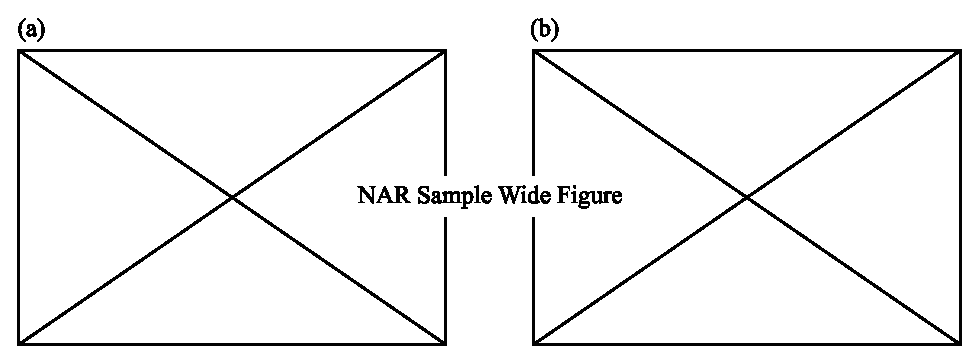
\includegraphics{NAR-fig2.eps}
\end{center}
\caption{Caption for wide figure over two columns.
\textbf{(a)} Left figure.
\textbf{(b)} Right figure (see (a)).
}
\label{NAR-fig2}
\end{figure*}


\subsection{Results subsection three}

Text. Text. Text. Text. Text. Text. Text. Text. Text. Text. Text.
Text. Text. Text. Text. Text. Text. Text. Text. Text. Text. Text.
Text. Text. Text. Text. Text. Text. Text. Text. Text. Text. Text.
Text. Text. Text. Text. Text. Text. Text. Text. Text. Text. Text.
Text. Text. Text. Text. Text. Text. Text. Text. Text. Text. Text.
Text. Text. Text. Text. Text. Text. Text. Text. Text. Text. Text.
Text. Text. Text. Text. Text. Text. Text. Text. Text. Text. Text.
Text. Text. Text. Text. Text. Text. Text. Text. Text. Text. Text.
Text. Text. Text. Text. Text. Text. Text. Text. Text. Text. Text.
Text. Text. Text. Text. Text. Text. Text. Text. Text. Text. Text.
Text. Text. Text.

\section{CONCLUSION}

Text. Text. Text. Text. Text. Text. Text. Text. Text. Text. Text.
Text. Text. Text. Text. Text. Text. Text. Text. Text. Text. Text.
Text. Text. Text. Text. Text. Text. Text. Text. Text. Text. Text.
Text. Text. Text. Text. Text. Text. Text. Text. Text. Text. Text.
Text. Text. Text. Text. Text. Text. Text. Text. Text. Text. Text.
Text. Text. Text. Text. Text. Text. Text. Text. Text. Text. Text.
Text. Text. Text. Text. Text. Text. Text. Text. Text. Text. Text.
Text. Text. Text. Text. Text. Text. Text. Text. Text. Text. Text.
Text. Text. Text. Text. Text. Text. Text. Text. Text. Text. Text.
Text. Text. Text.


\section{ACKNOWLEDGEMENTS}

Text. Text. Text. Text. Text. Text. Text. Text. Text. Text. Text.
Text. Text. Text. Text.


\subsubsection{Conflict of interest statement.} None declared.
\newpage


\begin{thebibliography}{4}

% Format for article
\bibitem{1}
Author,A.B. and Author,C. (1992)
Article title.
\textit{Abbreviated Journal Name}, \textbf{5}, 300--330.

% Format for book
\bibitem{2}
Author,D., Author,E.F. and Author,G. (1995)
\textit{Book Title}.
Publisher Name, Publisher Address.

% Format for chapter in book
\bibitem{3}
Author,H. and Author,I. (2005)
Chapter title.
In
Editor,A. and Editor,B. (eds),
\textit{Book Title},
Publisher Name, Publisher Address,
pp.\ 60--80.

% Another article
\bibitem{4}
Author,Y. and Author,Z. (2002)
Article title.
\textit{Abbreviated Journal Name}, \textbf{53}, 500--520.

\end{thebibliography}

\end{document}
